\noindent{\Huge Broad Phase}

W tej fazie wykrywa się jak najwięcej par obiektów, które na pewno się ze sobą nie zderzą, ponieważ np. są daleko od siebie. Obliczenia w tej fazie powinny być jak najprostsze, aby szybko i skutecznie odrzucić dużo par obiektów.

Algorytmy najczę\'sciej używane podczas Broad phase dzielą się na te, które dzielą lub układają przestrzeń i te, które po prostu porównują każdy obiekt z każdym poprzez otoczenie go jakim\'s kształtem.\\
Algorytmy, które opiszę, to:\begin{itemize}[topsep=0.2em, itemsep=0.5em, partopsep=0em, parsep=0em]
	\item AABB (Axis-Aligned Bounding Boxes)
	\item Bounding Boxes
	\item Bounding Circles
	\item Sweep and Prune
	\item Quadtree
	\item Octree
	\item Bounding Volume Hierarchy
	\item Bins
\end{itemize}
\bigskip
\noindent Czasami można w tej fazie użyć tymczasowej koherencji, czyli skorzystać z faktu, iż niektóre obiekty nie przesunęły się względem siebie od czasu ostatniego wykrywania kolizji, lub przesunęły się o względnie małą odległo\'sć, dzięki czemu od razu można je wykluczyć.\\

\noindent{\LARGE Bounding Volumes}\smallskip

Metody z grupy Bounding Volumes polegają na otoczeniu modelu jakim\'s prostym kształtem, i sprawdzaniu zderzeń tylko na tych kształtach. Są zazwyczej do\'sć proste do zaimplementowania i bardzo dobre je\'sli obiektów jest mało.\\

\noindent{\LARGE Space Partitioning}\smallskip

Druga grupa metod, wykorzystują one podział pola gry na obszary, zazwyczaj ułożone w strukturę drzewa. W każdym z pól każda para obiektów dla danego pola zostaje przetestowana czy została zderzona. Podział na obszary można zaimplementować na wiele sposobów.

\newpage
\noindent{\Large AABB (Axis-Aligned Bounding Boxes)}\smallskip

Metoda AABB polega na otoczeniu każdego obiektu prostokątem i sprawdzeniu które prostokąty się pokrywają.

Zaletami tej metody są łatwo\'sć implementacji, a także dokładno\'sć dla obiektów przypominających kształtem prostokąty wyrównane do osi.

Wadami tej metody są czas działania, czyli $O(n^{2})$ dla $n$ elementów, oraz fakt że dla pewnych obiektów jest ona bardzo niedokładna. Dla obracających lub zmieniających rozmiar obiektów trzeba też zmienić rozmiar prostokąta, co czasami może wymagać dużej ilo\'sci obliczeń, je\'sli model ma wiele wierzchołków.\\
Metody tej najlepiej używać, gdy obiektów jest niewiele i są one prostokątne (na przykład w platformówkach).
\begin{figure}[h]
	\centering
	\noindent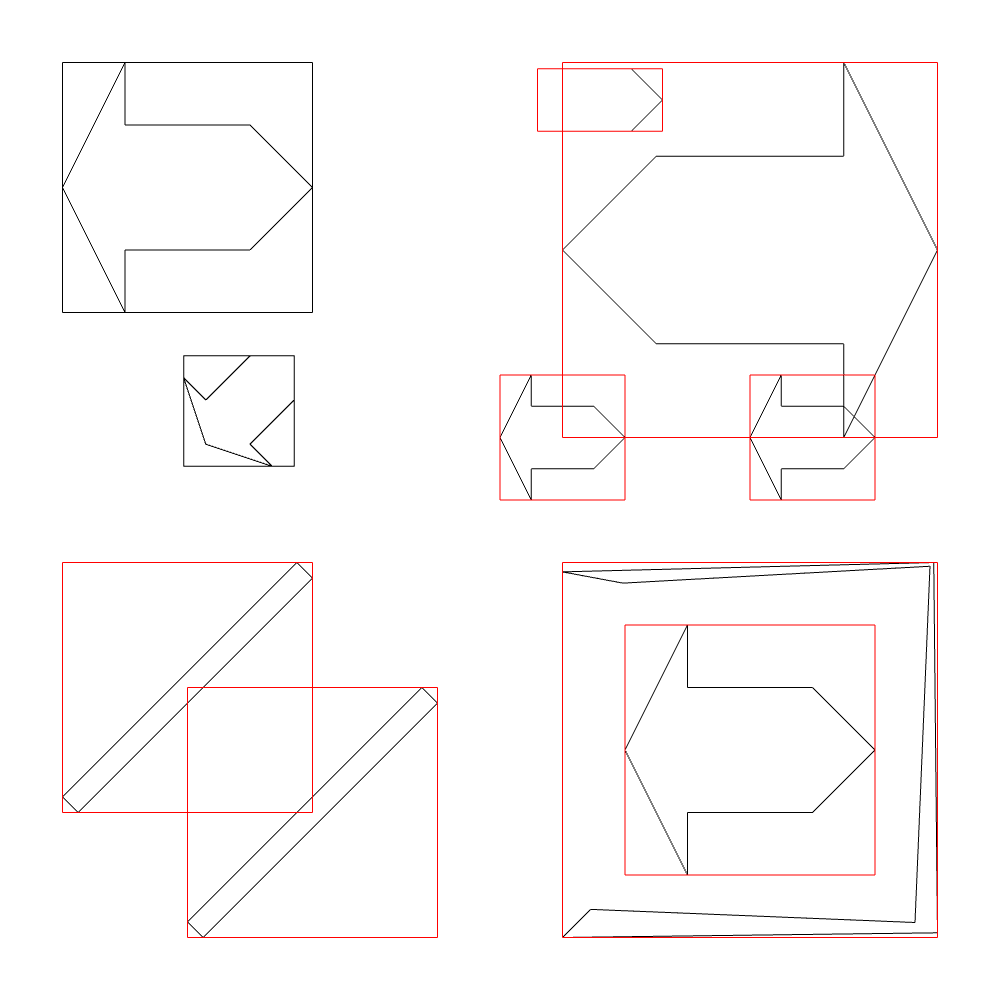
\includegraphics[width=0.84\textwidth]{collissionAABB}
	\caption{Przykład wykrywania kolizji metodą AABB, kolidujące obiekty są oznaczone na czerwono}
\end{figure}\\
Jak widać na obrazku, większo\'sć obiektów z czym\'s koliduje, ale pary obiektów będących daleko od siebie są odrzucone, co zdecydowanie zmniejsza liczbę obliczeń.
\newpage

\noindent{\Large Bounding Boxes}\smallskip

Ta metoda polega na otoczeniu każdego obiektu prostokątem, który nie musi być wyrównany do osi, w innych aspektach jest podobna do poprzedniej. Jest ona odrobinę trudniejsza do zaimplementowania, ale dzięki możliw\'soci obracania może być także dokładniejsza w niektórych przypadkach, a przy obrocie obiektu wystarczy obrócić odpowiadający mu prostokąt.

Wady tej metody to nieco większa złożono\'sć obliczeń, ciągle przy $O(n^{2})$ porównań.
\begin{figure}[h]
	\centering
	\noindent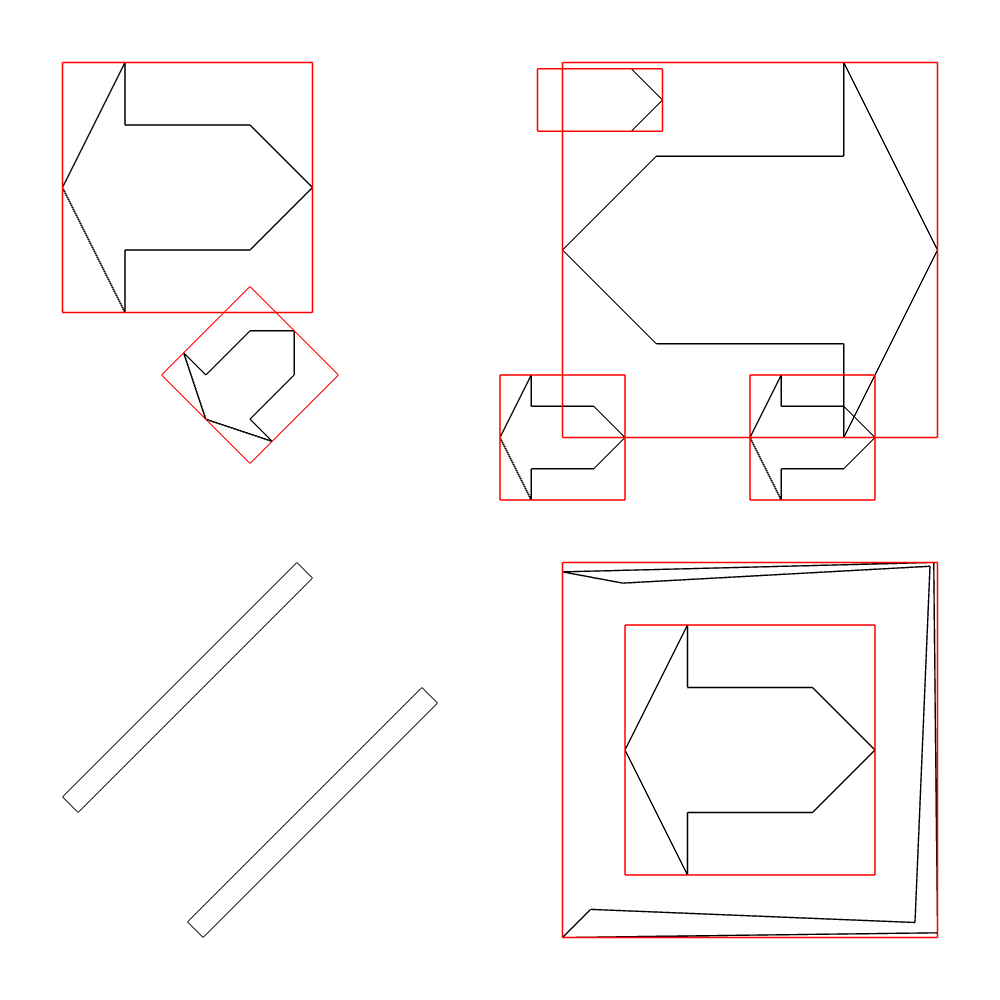
\includegraphics[width=\textwidth]{collission_rotated_boxes}
	\caption{Przykład wykrywania kolizji metodą Bounding Boxes}
\end{figure}\\
Patrząc na obrazek, w lewym dolnym rogu prostokąty odpowiadają teraz modelowi obiektu, ale za to w lewym górnym rogu widać, że tym razem program wykrył kolizję, której nie było w poprzednim przykładzie.
\newpage

\noindent{\Large Bounding Circles}\smallskip

Ta metoda jest podobna do dwóch poprzednich, ale tym razem używamy koła do sprawdzania możliwych zderzeń.

Plusami tej metody są łatwo\'sć jej zaimplementowania i bardzo mała ilo\'sć wymaganych danych oraz obliczeń: wystarczy tylko obliczyć odległo\'sc między dwoma obiektami i porównać z sumą ich promieni. Dodatkowo obrót obiektów i ich skalowanie nie wymusza obliczania danych na nowo, jesli używamy tej metody.

Wady tej metody to kiepska wydajno\'sć dla obiektów które są podłużne.
\begin{figure}[h]
	\centering
	\noindent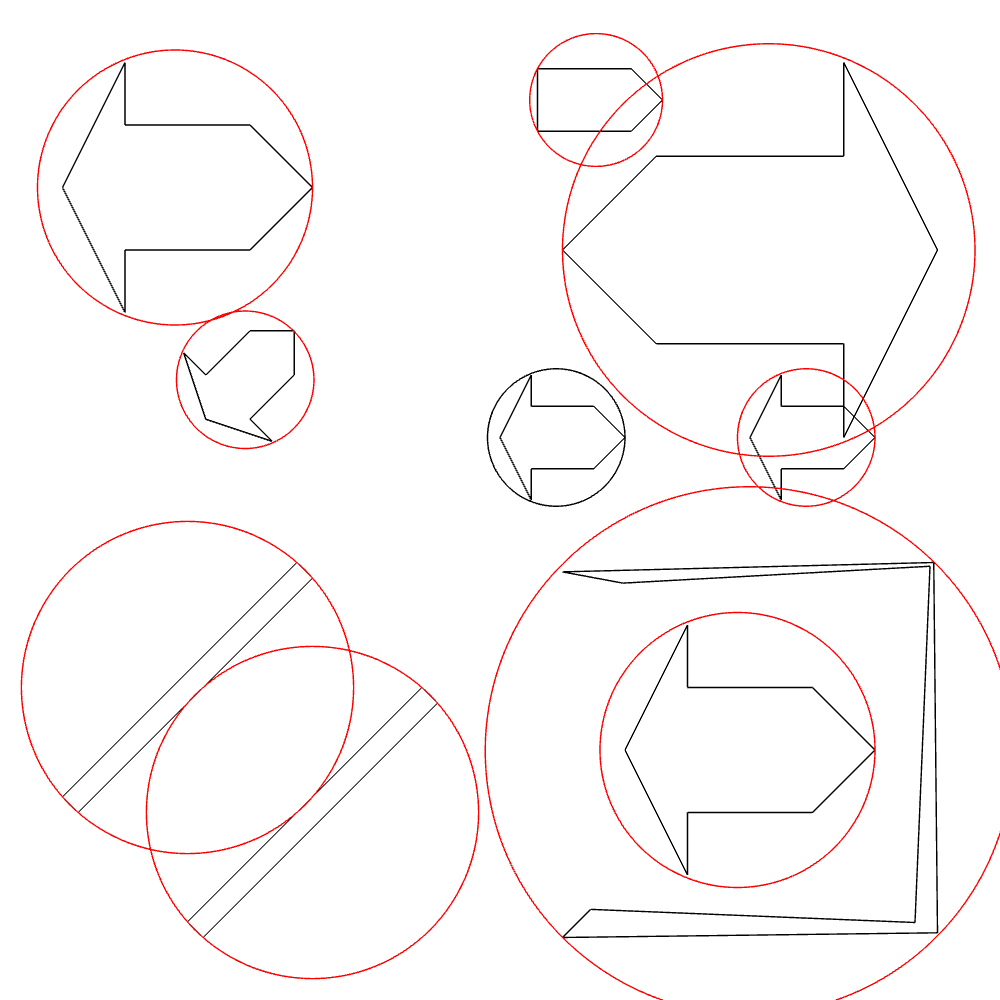
\includegraphics[width=\textwidth]{collission_circles}
	\caption{Przykład wykrywania kolizji metodą Bounding Circles}
\end{figure}\\
\newpage

\noindent{\Large Sweep and Prune}\smallskip

Metoda polegająca na posortowaniu obiektów względem położenia na osiach tych ich punktów, które są najbliżej i najdalej początku osi. Potem je\'sli początki i końce danej pary nakładają się na wszystkich osiach, to ta para przechodzi dany etap.

Zalety tej metody to szybszy czas działania, $O(nlogn)$ w porównianiu do $O(n^{2})$ poprzedniej metody.
\begin{figure}[h]
	\centering
	\noindent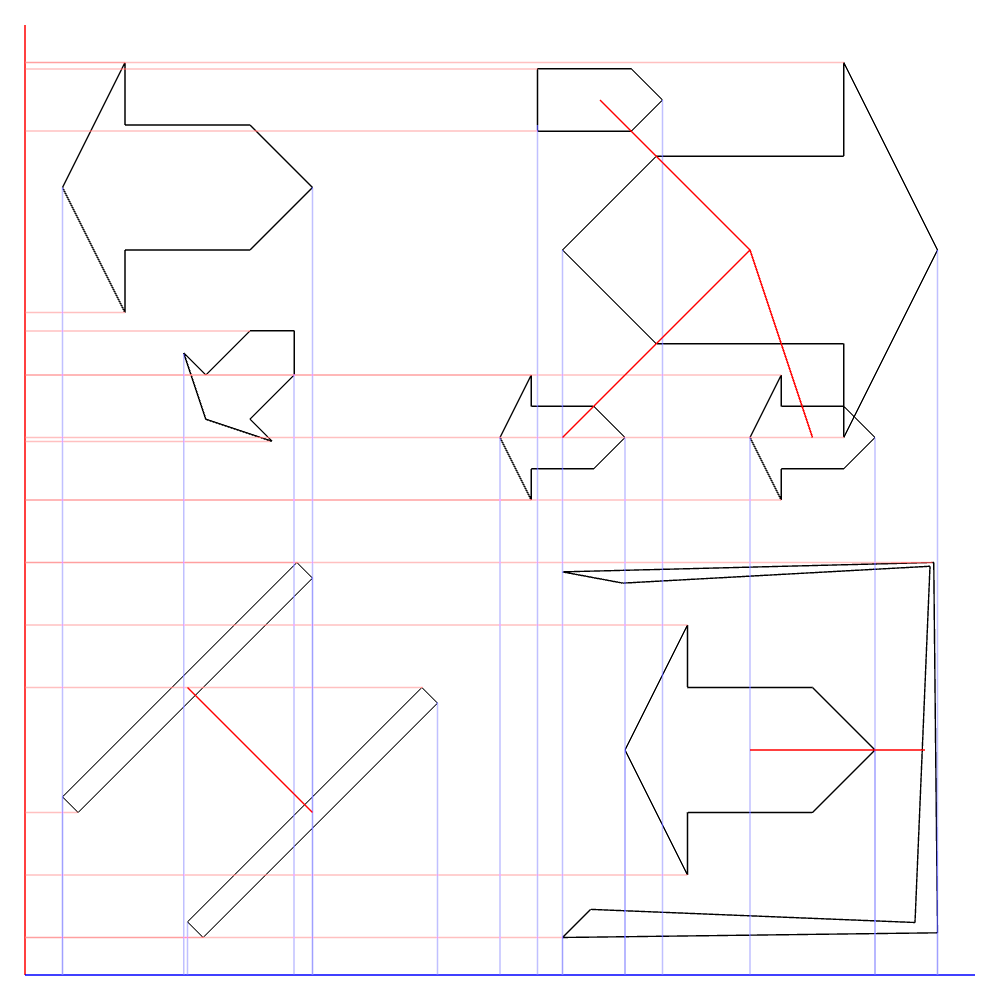
\includegraphics[width=\textwidth]{collission_sweep_and_prune}
	\caption{Przykład wykrywania kolizji metodą Sweep and Prune, kolizje są oznaczone czerwoną linią}
\end{figure}\\
Jak widać na obrazku, Wyniki są dokładnie takie same jak dla metody AABB, jednak czas działania tej metody jest dużo krótszy je\'sli niewiele elementów ze sobą koliduje.
\newpage

\noindent{\Large Quadtree}\smallskip

Każdy obszar jest kwadratem i może być podzielony na 4 podobszary, je\'sli zawiera odpowiednio małe elementy. Wykrywanie kolizji zachodzi gdy w jednym obszarze znajduje się więcej niż jeden obiekt.\\
\begin{figure}[h]
	\centering
	\noindent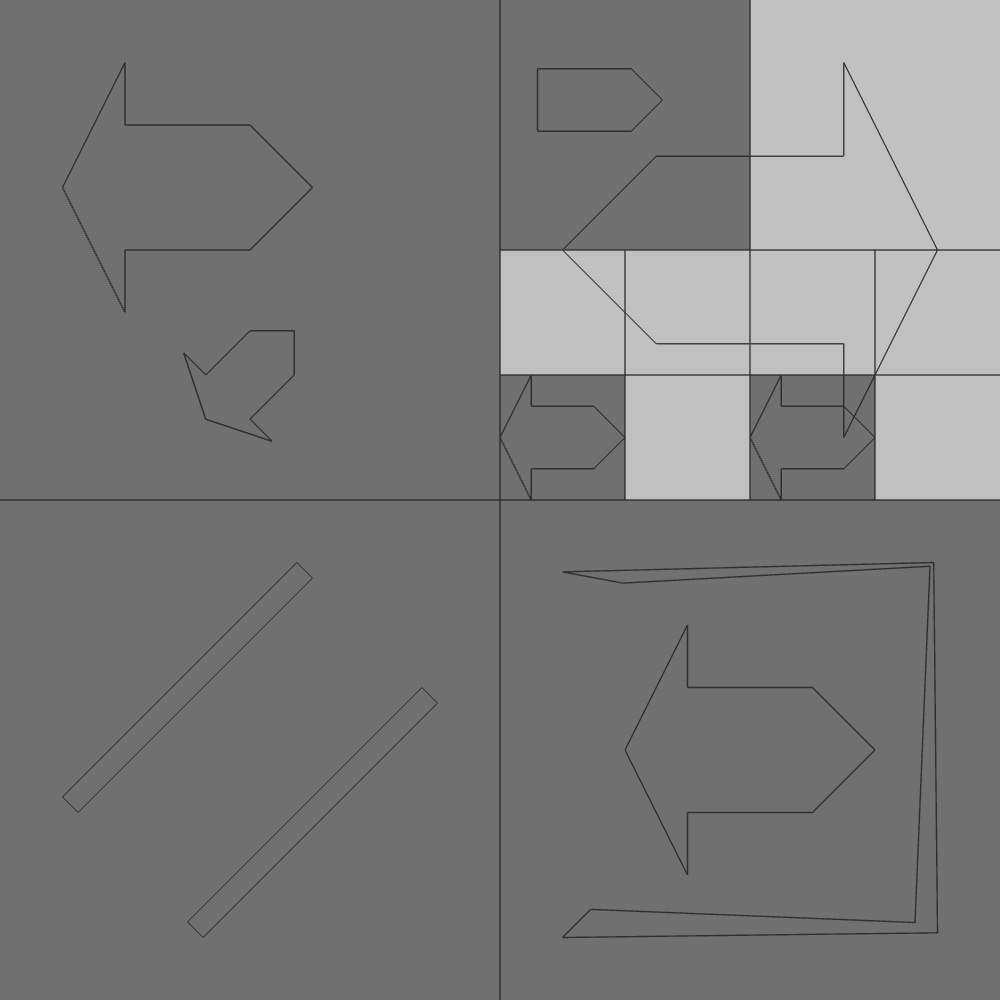
\includegraphics[width=\textwidth]{collission_quadtree}
	\caption{Przykład użycia metody Quadtree}
\end{figure}\\

\noindent{\Large Octree}\smallskip

Podobnie jak w Quadtree, Octree dzieli obszar na równej wielko\'sci podobszary, z tym że tutaj podział następuje w przestrzeni trójwymiarowej, sze\'scian dzieli się na 8 mniejszych sze\'scianów.\\
\newpage
 
\noindent{\Large Bounding Volume Hierarchy}\smallskip

Ta metoda tworzy drzewo przez połączenie dwóch drzew będących blisko siebie w jedno większe drzewo, którego będą poddrzewami. Obydwa poddrzewa w cało\'sci mieszczą się w obszarze będącym korzeniem drzewa. Tutaj kolizje zachodzą, je\'sli dwa poddrzewa się na siebie nakładają.\\
\begin{figure}[h]
	\centering
	\noindent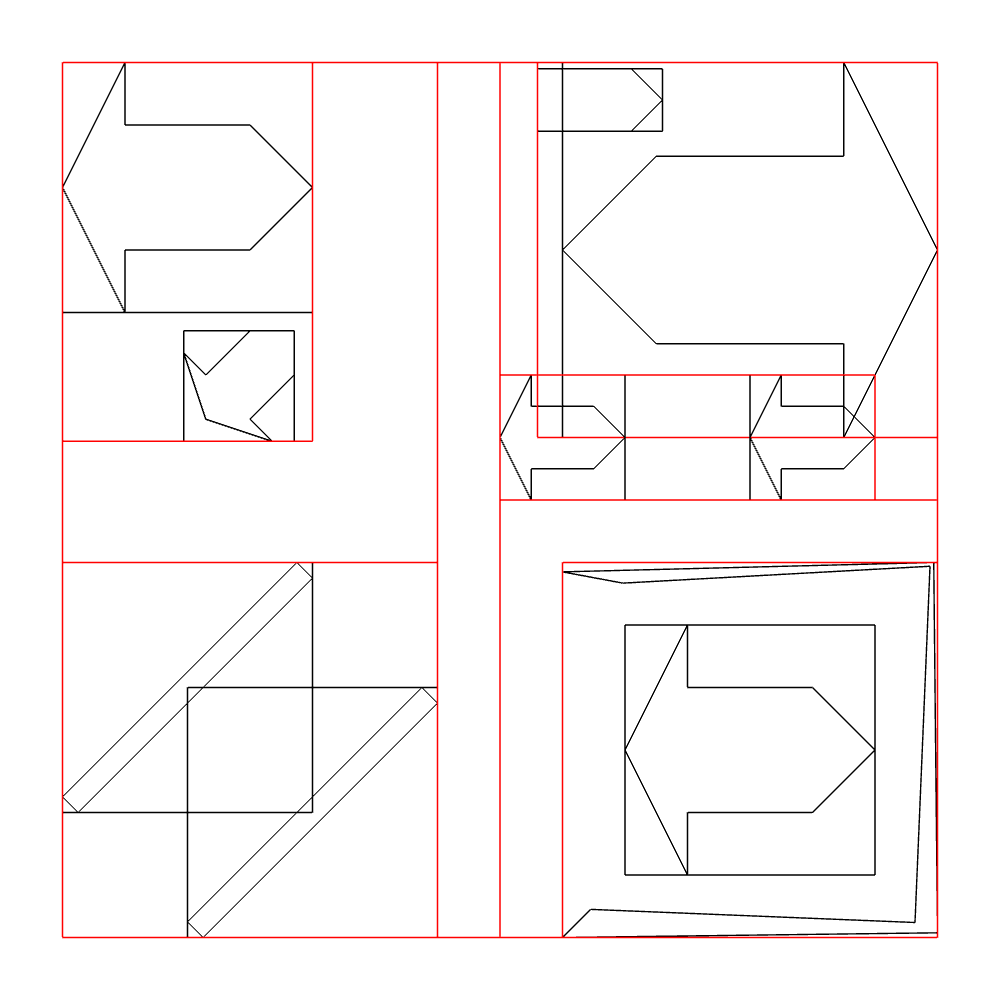
\includegraphics[width=\textwidth]{collission_bounding_volumes_hierarchy}
	\caption{Przykład użycia metody Bounding Volume Hierarchy}
\end{figure}\\
\newpage

\noindent{\Large Bins}\smallskip

Najprostsza z metod opartych na dzieleniu obszaru. Metoda ta dzieli obszar na wiele równych czę\'sci i do każdej z nich dodaje wszystkie obiekty które się z nią chociaż czę\'sciowo pokrywają. W danym obszarze kolizje liczone są w parach obiektów każdy z każdym.\\
\begin{figure}[h]
	\centering
	\noindent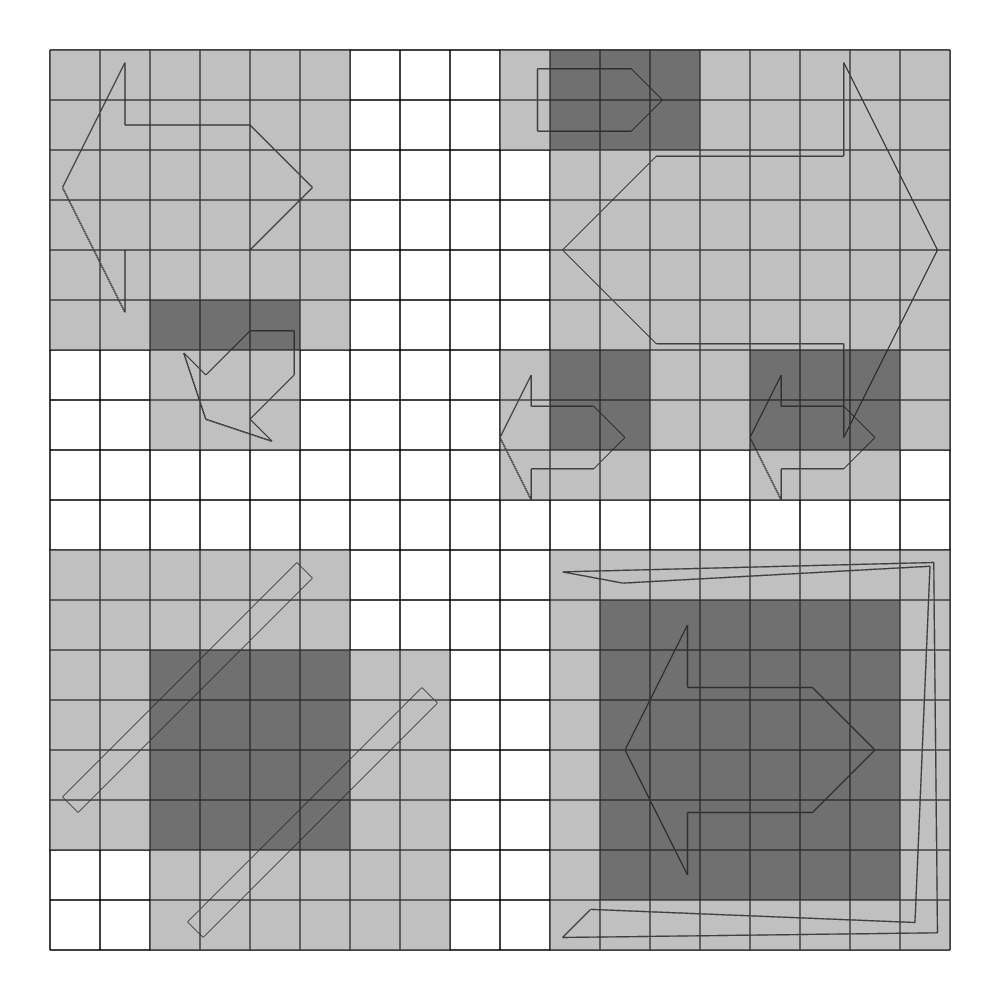
\includegraphics[width=\textwidth]{collission_bins}
	\caption{Przykład użycia metody , im pole ciemniejsze, tym więcej obiektów je pokrywa}
\end{figure}\\
\newpage